\documentclass[12pt,a4paper]{article}  % Déclare la classe du document.

\newcommand{\chaptermark}[2]{\og #2 \fg{} (#1)} % ligne uniquement pour éviter une erreur en cas d'article
\include{../1ere-preambule}

\usepackage{epic}   % extension et simplification de  l'environnement picture
\usepackage{graphicx}    % permet d'inclure des graphique externe dans un document
\usepackage{arydshln}   %permet d'avoir des lignes en pointillés

\newcommand{\lignes}[1]{
\setlength{\unitlength}{1mm}
\vskip 0,4cm\noindent
\multido{\i=0+1}{#1}{%
     \noindent
     \begin{picture}(150,5)
     \linethickness{0,005mm}
     \put(-5,0){\dashline{1}(175,5)(5,5)}
     \end{picture}\vskip 0,001cm
     }
\vskip 0cm
}

\rhead{Fiche d'exercices - Appl. Produit Scalaire}

\begin{document}
\graphicspath{{images/}}

\begin{center}
\fbox{
\begin{minipage}[]{15cm}
\begin{center}
\LARGE{\rule{0.5cm}{0pt}\rule[-0.25cm]{0pt}{0.9cm}
Fiche d'exercices\\
Application produit scalaire
}
\end{center}
\end{minipage}
}

\end{center}


% \begin{center}\textbf{2h - Calculatrice autorisée - Barème indicatif}\end{center}

% %\begin{center}\textbf{Les élèves avec un tier-temps ne traitent pas les questions avec  le symbole \ding{46}}\end{center}

% \begin{center}
% %On veillera à ENCADRER ses résultats et soigner sa copie.\\
% Les résultats doivent être justifiés par des calculs (au moins 1 étape intermédiaire).
% \end{center}

\exerciceDS{}
$\mathrm{ABC}$ est un triangle tel que :$A B=2, A C=6 \text { et } \widehat{B A C}=60^{\circ} .$\\
Calculer la valeur exacte de la longueur $B C$.


\exerciceDS{}
ABCD est un parallélogramme tel que :$A B=6, A D=4 \text { et } \widehat{D A B}=60^{\circ} .$
\begin{multicols}{2}
\begin{enumMet}
    \item Construire une figure.
    \item Calculer la longueur BD.
    \item Quelle est la mesure de l'angle $\widehat{A B C}$ ?
    \item Calculer la longueur AC.
\end{enumMet}
\end{multicols}

\vspace{-0.3cm}
\exerciceDS{}

\begin{minipage}[c]{0.55\linewidth}
Un voilier V approche de la côte. Il est situé à 9 milles du phare A, à 5 milles du phare $B$ et l'angle $\widehat{AVB}$ mesure $60^{\circ} .$
Calculer la distance AB entre les deux phares. Arrondir au dixième.
\end{minipage} \hfill
\begin{minipage}[c]{0.4\linewidth}
\begin{center}
    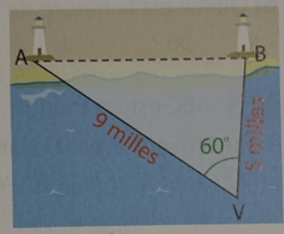
\includegraphics[scale=0.9]{../images/1.06.04 - Img01.png}
\end{center}
\end{minipage}

\exerciceDS{}
Dans les 2 cas ci dessous, calculer $\vv{A B} \cdot \vv{A C}$.
\begin{multicols}{2}
\begin{enumMet}
    \item \ \\
    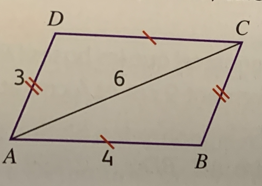
\includegraphics[scale=1.2]{../images/1.06.04 - Img02.png}
    \item \ \\
    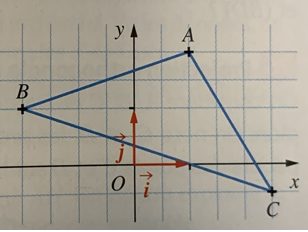
\includegraphics[scale=1.2]{../images/1.06.04 - Img03.png}
\end{enumMet}
\end{multicols}

\exerciceDS{}
On considère deux vecteurs $\vv{u}$ et $\vv{v}$ du plan tels que $\|\vv{u}+\vv{v}\|=5$ et $\|\vv{u}-\vv{v}\|=3$. Calculer le produit scalaire $\vv{u} \cdot \vv{v}$.

\exerciceDS{}
Dans le plan muni d'un repère orthonormé, on considère les vecteurs
$\Coord{u}{2}{-3}$ et $\Coord{v}{1}{2}$.
\begin{enumMet}
    \item calculer $\vv{u} \cdot \vv{v},\|\vv{u}\|$ et $\|\vv{v}\|$.
    \item Calculer de deux façons les nombres : $\|\vv{u}+\vv{v}\|^{2} \text { et }\|\vv{u}-\vv{v}\|^{2}$
    \item Calculer de deux façons $(\vv{u}+\vv{v}) \cdot(\vv{u}-\vv{v})$.
\end{enumMet}

\exerciceDS{}
Le plan est muni d'un repère orthonormé. Dans chaque cas, calculer $\vv{A B} \cdot \vv{A C}$ puis une mesure (arrondie au degré près) de l'angle $\widehat{B A C}$.
\begin{enumMet}
    \item $A(-1 ; 4), B(2 ; 2)$ et $C(1 ; 5)$
    \item $A(2 ; 4), B(1 ; 3)$ et $C(4 ; 2)$
    \item $A(0 ; 4), B(-3 ; 5)$ et $C(6 ; 2)$
\end{enumMet}


\exerciceDS{}
Dans un repère orthonormé du plan, on considère les points $A(1 ; 4), B(-3 ;-2)$ et $C(2 ;-5)$.\\
Déterminer les angles du triangle $A B C$ à 0,1 degré près.

\exerciceDS{}
$A B C$ est un triangle tel que $A B=4, A C=3$ et $\widehat{B A C}=135^{\circ} . M$ est le milieu du segment $[A C]$ et $P$ est le point déini par $\vv{A P}=\frac{3}{4} \vv{A B}$.
\begin{enumMet}
    \item En notant que $\vv{M P}=\vv{A P}-\vv{A M}$, calculer $\vv{M P^{2}}$.
    \item En déduire la longueur $M P$.
\end{enumMet}

\exerciceDS{}
$A B C D$ est un parallélogramme tel que $A B=3$, $A D=5$ et $A C=6$.
\begin{enumMet}
    \item 1. Rappeler la formule exprimant $\vv{u} \cdot \vv{v}$ en fonction de $\|\vv{u}\|,\|\vv{v}\|$ et $\|\vv{u}+\vv{v}\|$.\\
    Calculer alors le produit scalaire $\vv{A B} \cdot \vv{A D}$.
    \item En déduire une mesure, en degré, de l'angle $\widehat{B A D}$ (on donnera une valeur arrondie au degré près).
\end{enumMet}

\exerciceDS{}
$A B C D$ est un parallélogramme tel que $A B=4$, $A D=6$ et $\widehat{B A D}=40^{\circ}$.\\
Calculer le produit scalaire $\vv{A B} \cdot \vv{A C}$ (on pourra décomposer le vecteur $\vv{A C}$ ).





\end{document}

